\documentclass[12pt]{article}

\usepackage{amsmath, mathtools, amssymb}
\usepackage[margin=0.5in]{geometry}
\usepackage[document]{ragged2e}
\usepackage{tikz}
\usepackage{undertilde}
\newcommand{\vect}[1]{\boldsymbol{#1}}

\usepackage{graphicx} % \scalebox
\usepackage{environ}
\NewEnviron{largeMath}{%
\begin{equation}
\scalebox{1.5}{$\BODY$}
\end{equation}
}

\makeatletter
\renewcommand*\env@matrix[1][*\c@MaxMatrixCols c]{%
  \hskip -\arraycolsep
  \let\@ifnextchar\new@ifnextchar
  \array{#1}}
\makeatother
\newcommand{\norm}[1]{\left\lVert#1\right\rVert}

\begin{document}
Vector Calculus Mast 20009 \hfill Felix McCuaig, 1159424 \\
Assignment 3 \hfill Tutorial Wed 5:15PM
\section*{Question 1}
Let $S$ be the surface given by
$$
x^2+2y^4+3z^6=1 \text{ with } z \geqslant 0.
$$
Let $\Gamma$ be the curve
$$
\gamma (t)= \left( \cos(\pi t) , \sqrt{t+1}, \frac{2t}{t^2+1} \right), \hspace{20px} \text{ for } \hspace{20px}  0 \leqslant t \leqslant 1
$$
and let $\mathbf{F}$ be the vector field 
$$
\mathbf{F}(x,y,z)=(a-4z^2x)\vect{i}+2by\vect{j}+cx^2z\vect{k}
$$
where $a,b,c \in \mathbb{R}$\\
\medskip
\textbf{(a)} Compute
$$
\iint_{S}(\nabla \times \mathbf{F})\cdot d \vect{S}.
$$
According to Stokes' theorem:
$$
\iint_{S}(\nabla \times \mathbf{F})\cdot d \vect{S}=\int_{\partial S}\mathbf{F}\cdot d \vect{S}.
$$
Where $\partial S$ is the boundary of $S$, which occurs when $z = 0$. Hence, $\partial S$ is given by:
$$
x^2+2y^4=1
$$
Now, $\partial S$ should parametrised:\\
$$
x = \pm \cos t, \hspace{20px} y = \pm \frac{\sqrt{\sin t}}{\sqrt{\sqrt{2}}}, \hspace{20px} z = 0
$$
To verify:
$$
=\cos^2 t + 2 \left( \frac{\sin t}{\sqrt{2}} \right)^2
$$
$$
=\cos^2 t + 2 \sin^2 t
$$
$$
=1
$$
Nice, now we need to traverse our squary ellipsey thing in an anticlockwise direction: \\
\smallskip
That is, for $(x, y, z):$
$$(1,0,0)\rightarrow(-1,0,0)\rightarrow(1,0,0)$$
When $\cos t = 1, t = 0$, when $\cos t = -1, t = \pi$. \\
Since $y$ has a $\pm$ thingy, we should traverse the curve in two segments: \\
$$
\mathbf{p}_1(t)=\left(\cos t, \frac{\sqrt{\sin t}}{\sqrt{\sqrt{2}}} , 0\right) t \in [0, \pi]
$$

$$
\mathbf{p}_2(t)=\left(-\cos t, -\frac{\sqrt{\sin t}}{\sqrt{\sqrt{2}}}, 0\right) t \in [0, \pi]
$$
\begin{center}
  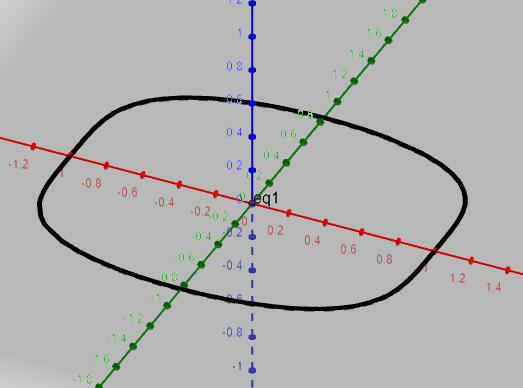
\includegraphics{capture1}
\end{center}
Note: $d \mathbf{S}_1$ corresponds to $\mathbf{p}_1$ and  $d \mathbf{S}_2$ to $\mathbf{p}_2$
$$
\int^{\pi}_{0}\mathbf{F}\left(\cos t, \frac{\sqrt{\sin t}}{\sqrt{\sqrt{2}}}, 0\right)
\cdot
d \mathbf{S}_1
-\int^{\pi}_{0}\mathbf{F}\left(-\cos t, -\frac{\sqrt{\sin t}}{\sqrt{\sqrt{2}}}, 0\right)
\cdot
d \mathbf{S}_2
$$
Note, the integrals must be subtracted or we get $0$. \\
\medskip
If we take out the negatives from our second integral we have twice our first 
integral. So let's just do the integral once and double it later.\\
Now, we know that $d \mathbf{S}$ is:
$$
d\mathbf{S}= \left( \frac{\partial x}{\partial t}, \frac{\partial y}{\partial t}, \frac{\partial z}{\partial t}\right) dt
$$
$$
d\mathbf{S}_1=
\left( 
  -\sin t, 
  \frac{1}{2}\times\frac{\cos t}{\sqrt{2}}\times\left( \frac{\sin t}{\sqrt{2}}\right)^{-\frac{1}{2}}, 
  0
\right)dt
$$
$$
\mathbf{F}(\mathbf{c}(t))=
\left( 
  a-4(0)^2\cos t,
  2b \times \left( \frac{\sin t}{\sqrt{2}} \right)^{\frac{1}{2}},
  0
\right)
=
\left( 
  a,
  2b \left( \frac{\sin t}{\sqrt{2}} \right)^{\frac{1}{2}},
  0
\right)
$$
$$
\int^{\pi}_{0}
\left( 
  a,
  2b \left( \frac{\sin t}{\sqrt{2}} \right)^{\frac{1}{2}},
  0
\right)
\cdot
\left( 
  -\sin t, 
  \frac{\cos t}{2\sqrt{2}}\left( \frac{\sin t}{\sqrt{2}}\right)^{-\frac{1}{2}}, 
  0
\right)dt
$$
$$
\int^{\pi}_{0}
-a\sin t + \frac{b}{\sqrt{2}}\cos t \
dt
$$
$$
\left[
  a\cos t + \frac{b}{\sqrt{2}}\sin t
\right]^{\pi}_{0}=-2a
$$
Now, let's double our result (yielding our final answer):
$$
\therefore \iint_{S}(\nabla \times \mathbf{F})\cdot d \vect{S} = -4a
$$
\medskip
\textbf{(b)} Find all values of $a, b$ and $c$ such that the vector field $\mathbf{F}$ is conservative.\\
\smallskip
Since 
$$
\iint_{S}(\nabla \times \mathbf{F})\cdot d \vect{S}=\int_{\partial S}\mathbf{F}\cdot d \vect{S}.
$$
Our vector field $\mathbf{F}$ is conservative when:
$$
\iint_{S}(\nabla \times \mathbf{F})\cdot d \vect{S}=0.
$$
Therefore $a=0, \hspace{5px} b \in \mathbb{R} \hspace{5px} c \in \mathbb{R}$.\\
Note, this visually makes sense as when $a=0$, the vector field is symmetric upon all axes, but
when $a\neq 0$, it's wonky (technical term for asymmetric).\\
\medskip
\textbf{(c)} If $a,b,c$ are chosen such that $\mathbf{F}$ is conservative, 
compute the work done by $\mathbf{F}$ to move a particle along $\Gamma$ in the direction of increasing $t$.\\
\smallskip
To choose $a,b,c$ such that $\mathbf{F}$ is conservative, let $a=0, \hspace{5px} b \in \mathbb{R} \hspace{5px} c \in \mathbb{R}$.
Then, $\mathbf{F}$ is:
$$
\mathbf{F}(x,y,z)=(-4z^2x)\vect{i}+2by\vect{j}+cx^2z\vect{k}
$$
We want to calculate the work done as $t\in [0, 1]$.
\end{document}